\chapter{Free to Choose}

We begin where the previous lecture left off. John Stuart Mill had tried to save utilitarianism by distinguishing higher from lower pleasures, and by suggesting that justice and rights could also be vindicated within a broadly utilitarian framework. In this lecture Michael Sandel presses that attempt from several directions, then turns to libertarianism as a strong theory of rights. The lecture becomes increasingly explicit in its structure: first the pressure on Mill, then the libertarian account of liberty, then the institutional consequences for law and the state, and finally the deeper question of self-possession that will carry us to Locke.

\section{From Mill's Repair to the Problem of Rights}

Sandel does not start with libertarianism. He first reopens the unresolved problem from the previous meeting. Mill wanted to say that one can remain within utilitarianism and still distinguish qualitatively better pleasures from worse ones. But the classroom experiment had produced an awkward result: many students preferred one thing while still judging another to be worthier.

A compact way to display the tension is the following:
\begin{equation}
\text{Preferred} \neq \text{Worthier}.
\end{equation}
This is not Mill's own notation; it is a schematic way to mark the instability in his defense of higher pleasures. Once that instability is on the table, Sandel shifts from pleasures to rights and justice.

Mill, on this second front, wants to say that rights are not peripheral but central. Justice is the most sacred and binding part of morality. Sandel grants, for the sake of argument, the form of Mill's reply:
\begin{equation}
\text{Respect rights} \Longrightarrow \text{better social consequences in the long run}.
\end{equation}
Again, the lecture gives this as prose rather than as formula, but the conditional structure is unmistakable. The point of the section is that even if we grant the long-run calculation, two worries remain.

The first worry is about exceptions. If violating a right in some case really would improve things in the long run, would utilitarianism then permit the violation after all? The second worry is deeper. Even if respecting rights always did improve the long-run welfare of society, would that be the right moral explanation of why we must not use persons?

To make the second worry vivid, Sandel returns to the organ-transplant case. Suppose the doctor refrains from taking organs from the healthy patient because doing so would eventually damage public trust in medicine. That answer may point to bad consequences. But Sandel asks whether there is another reason, namely, that the patient must be respected as a person and not treated as available material for a social purpose.

\subsection{Question \& Answer}

The lecture raises the question in a sharp form: if respecting rights makes society better off in the long run, is that the right reason to respect persons?

The answer developed here is negative. A merely instrumental defense of rights does not yet capture what is morally weighty about them. The point of the organ-transplant example is not only that utilitarianism may misfire in hard cases; it is also that the language of aggregate welfare may fail to name the right kind of reason. This is the moment at which the lecture needs a stronger theory of rights.

\section{Libertarianism as a Strong Theory of Rights}

Sandel's transition is deliberate. If Mill's utilitarianism seems to lean, perhaps covertly, on dignity or respect for persons, then we should ask whether there are theories that make those ideas primary rather than derivative. That is how libertarianism enters the lecture.

The central thought is that persons are separate beings with separate lives. They are not simply sites at which satisfactions are stored and later added together. A strong theory of rights therefore treats it as a mistake to think about justice only by aggregating preferences and values.

Libertarianism takes the basic right to be liberty. Because we are separate persons, we are not available for use by society at large, even when that use is said to serve a worthy social purpose. In schematic form, the lecture pushes toward the following idea:
\begin{equation}
\text{SelfOwnership}(p)\Longrightarrow \text{strong side-constraints on using }p.
\end{equation}

This is the background of Nozick's famous formulation that individual rights are so strong and far-reaching that they raise the question of what, if anything, the state may do. Sandel's next move is therefore not to linger in abstraction. He asks what this doctrine means institutionally.

\section{The Minimal State and Its Three Prohibitions}

Once liberty is taken as fundamental, the lecture translates principle into policy. Sandel presents three kinds of state action that libertarianism rejects.

\begin{enumerate}
\item Paternalist legislation, laws that protect people from themselves.
\item Morals legislation, laws that try to promote virtue or enforce a shared moral view.
\item Redistribution, taxation or policy aimed at transferring income or wealth from the rich to the poor.
\end{enumerate}

The lecture's order matters. Seatbelt laws and helmet laws illustrate paternalism. Traditional restrictions on consensual sexual intimacy illustrate morals legislation. Redistribution then becomes the most developed case, because it brings into focus both coercion and property.

A useful schematic summary is
\begin{equation}
S_{\mathrm{forbidden}}=\{\text{paternalism},\ \text{morals legislation},\ \text{redistribution}\}.
\end{equation}
Against this, the minimal state is allowed a very narrow range of functions:
\begin{equation}
S_{\min}=\{\text{defense},\ \text{police},\ \text{courts},\ \text{contract/property enforcement}\}.
\end{equation}

That set notation is editorial, not spoken by Sandel. But it captures the form of the doctrine as it is introduced in the lecture. The important feature is not the symbolism itself, but the way the lecture unfolds the implications of liberty: no coercion for our own good, no coercion for virtue, and no coercion for redistributive equality.

\section{Redistribution, Historical Justice, and the Entitlement View}

Sandel now narrows to the third prohibition. He asks whether the distribution of wealth in the United States is just or unjust. The crucial libertarian reply is that we cannot tell merely by looking at the pattern.

We therefore introduce a bit of notation for the lecture's historical idea:
\begin{equation}
J(D)\ \text{depends on the history of acquisition and transfer, not on pattern alone}.
\end{equation}
Here \(D\) denotes a distribution or end-state of holdings, and \(J(D)\) denotes its justice-status. The guiding thought is that a distribution is not judged by how equal or unequal it looks at the end, but by how it came about.

Sandel then states the two principles we must examine:
\begin{enumerate}
\item justice in acquisition, whether the initial holdings were obtained justly;
\item justice in transfer, whether later holdings arose from voluntary exchange.
\end{enumerate}

A compact reconstruction is
\begin{equation}
J(D)=J_{\mathrm{acq}} \land J_{\mathrm{tr}}.
\end{equation}
This is again a schematic compression of the lecture's prose. It says: if the initial holdings were just, and if the later transfers were free and legitimate, then the resulting distribution is just; if not, it is unjust.

\subsection{Question \& Answer}

Can we judge a distribution by the end-state alone, or only by its history?

The answer in this part of the lecture is clear. Libertarian justice is historical rather than patterned. A society may be highly unequal and yet, on this view, just, if its holdings arose through just acquisition and voluntary transfer. Conversely, a more equal society may still be unjust if the route by which it reached that pattern involved theft, coercion, or expropriation.

\section{Bill Gates, Michael Jordan, and the Argument in Numbers}

At this point Sandel makes the issue concrete. He turns to Bill Gates and Michael Jordan not as current economic data points but as lecture-era examples that force the issue of redistribution.

The Gates example is designed to activate utilitarian intuition. If one person is so rich that losing a small amount would barely register, while many poor people could be significantly helped by receiving it, then redistribution seems immediately attractive. Sandel heightens the point with a few quantitative illustrations: Gates could afford an extraordinary number of Lincoln Bedroom stays, and his effective earning rate is said to exceed \$150 per second. So much so, Sandel jokes, that a \$100 bill on the street would not be worth the time required to stop and pick it up.

The Jordan example is even more useful for the notes because it becomes a worked numerical case. Sandel gives Jordan's yearly income as
\begin{equation}
31\,\text{million}+47\,\text{million}=78\,\text{million}.
\end{equation}
He then asks us to imagine requiring Jordan to pay roughly a third of that total to support food, health care, housing, and education for the poor. The implied arithmetic is straightforward:
\begin{equation}
\frac{1}{3}\cdot 78\,\text{million}=26\,\text{million}.
\end{equation}

\paragraph{Worked example.}
The lecture's utilitarian and libertarian reactions can be displayed side by side.
\begin{enumerate}
\item Start with Jordan's total income, \(78\) million dollars.
\item Take a third, yielding \(26\) million dollars.
\item A utilitarian says: the loss to Jordan is marginal, the gain to those in need is large.
\item A libertarian says: the calculation of benefit does not settle the moral question, because if the money is his by right, taking it is coercive.
\end{enumerate}

This is where the classroom dialectic begins in earnest. Sandel invites objections and replies. Some students argue that great wealth reflects social support and carries social obligation. Others argue that the poor need the money more, or that equality of opportunity breaks down when wealth becomes too concentrated. At this stage the lecture is not yet resolving those objections; it is organizing them.

A distinction that becomes important in the discussion is the difference between need and desert. One may need help desperately without thereby being entitled, on libertarian premises, to holdings that belong to another. The lecture does not convert this into formal symbolism, but it is useful to keep the distinction conceptually sharp.

\section{Taxation, Forced Labor, and Self-Possession}

Sandel now presses the libertarian case in its strongest Nozickian form. Joe's skateboard analogy introduces the theme by comparing redistributive taking to the unjust seizure of privately held goods. But Sandel then goes beyond the analogy, because Nozick's real argument is not merely that redistribution is theft.

The deeper chain is
\begin{align}
\text{taxation of earnings}
&\to \text{taking fruits of labor} \\
&\to \text{claim on labor} \\
&\to \text{forced labor} \\
&\to \text{slavery}.
\end{align}

The lecture's claim is that if the state may rightfully take the earnings produced by my labor, then it is asserting a claim on the labor that produced those earnings. And if it may claim some of my labor, then it is, in part, owner of me. That is why Sandel says the stakes are so high: redistribution is no longer being described merely as inefficient or even merely as theft, but as morally akin to slavery.

\begin{figure}
\centering
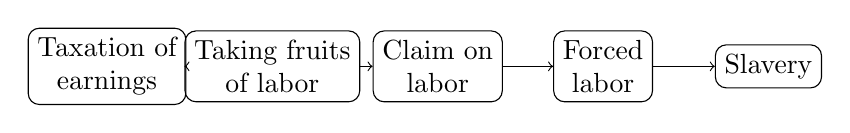
\begin{tikzpicture}[node distance=2.1cm, every node/.style={draw, rounded corners, align=center}]
\node (a) {Taxation of\\earnings};
\node (b) [right of=a] {Taking fruits\\of labor};
\node (c) [right of=b] {Claim on\\labor};
\node (d) [right of=c] {Forced\\labor};
\node (e) [right of=d] {Slavery};
\draw[->] (a) -- (b);
\draw[->] (b) -- (c);
\draw[->] (c) -- (d);
\draw[->] (d) -- (e);
\end{tikzpicture}
\end{figure}

The diagram is not a reproduction of any board image; it is a clean rendering of the lecture's logical sequence. Sandel then identifies the hidden premise that makes the entire argument move:
\begin{equation}
\text{SelfOwnership}(p)\Longrightarrow \text{the state has no claim on the labor of }p.
\end{equation}

This premise also explains the lecture's return to the organ-transplant case. If we own ourselves, then we are not available either for organ harvesting, or for paternalistic legislation, or for moral tutelage, or for redistributive use in the name of the common good. The same principle is doing the work in every case.

\subsection{Question \& Answer}

Is taxation for redistribution really morally equivalent to forced labor?

Sandel does not simply answer yes and move on. He first gives the strongest libertarian chain that yields that result. Then he invites resistance. Some students say the argument mistakes democratic taxation for slaveholding. Others say the successful owe a debt to the society that made their success possible. Still others say that need and equality of opportunity matter. The lecture's pedagogical point is that if we want to reject the conclusion, we must find the precise link in the chain where we part company with it.

\section{The Reprise: Minimal State, Democracy, and the Turn to Locke}

At this point the lecture undergoes a functional reset. Sandel explicitly returns to libertarianism and says that before resuming redistribution, he wants to say a word about the minimal state. This reprise is not redundant; it sharpens the institutional implications of the doctrine.

Milton Friedman is introduced to extend the anti-paternalist point. Even Social Security, on this view, is suspect, because however sensible retirement saving may be, it is wrong for the state to compel everyone to save. People should be free to choose badly as well as wisely, and liberty includes the liberty to take risks with one's own future.

The Salem Fire Corporation anecdote serves a similar purpose. It is a way of showing that what many people treat as necessarily public goods can, at least in principle, be privatized and restricted to subscribers. Sandel does not present this as a piece of mathematics, and we should not overformalize it. Its function is conceptual: to widen the scope of what the minimal-state view is willing to privatize.

Sandel then stages a more organized encounter between Team Libertarian and the objections already circulating in class. The objections come in a sequence:
\begin{enumerate}
\item the poor need the money more;
\item taxation by democratic consent is not slavery;
\item the successful owe a debt to society.
\end{enumerate}
The libertarian replies come in a matching sequence:
\begin{enumerate}
\item benefit does not justify violation of property right;
\item majority rule does not nullify a fundamental right;
\item social benefit already received through voluntary exchange cancels any supposed further debt.
\end{enumerate}

The democracy exchange is especially important. Alex insists that having a tiny share in a vote is not the same as deciding for oneself how to use one's property. Sandel then presses him with the possibility of democratic persuasion, and the reply becomes more refined: democracy is acceptable, but only within constitutional limits that prevent majorities from voting away fundamental rights. Sandel strengthens the point by comparing property claims with rights such as freedom of speech and religious liberty.

The last and most important objection comes from Victoria. Perhaps, she says, living in society already means that we do not own ourselves in the full libertarian sense. If we may not kill those who offend us, if we must account for others around us, and if wealth is never wholly our own doing, then maybe self-possession is not the moral primitive that libertarianism assumes.

That objection leads Sandel to the lecture's final transition. Nozick does not create the idea of self-possession from nothing. He inherits it from Locke. The closing chain is therefore not a conclusion but a preview:
\begin{equation}
\text{self-possession}\to \text{ownership of labor}\to \text{mixing labor with unowned things}\to \text{private property}.
\end{equation}

The lecture ends by asking us to follow that chain into the next chapter. If the libertarian critique of redistribution depends on self-ownership, and if self-ownership depends on a Lockean picture of the person and of labor, then the next task is clear: we must examine Locke.

\section{Summary}

The lecture begins as a criticism of Mill and ends as a challenge to the deepest premise of libertarianism. Along the way Sandel preserves a precise order of discovery. We first see why a long-run utilitarian defense of rights is unstable. We then turn to libertarianism as a strong theory of rights, derive its minimal state, and sharpen its historical account of justice. After that, concrete examples of Gates and Jordan force the redistributive question into the open, and Nozick's argument drives the issue down to self-possession.

The result is not closure but concentration. The real issue is no longer simply whether redistribution is wise, or compassionate, or democratically authorized. The real issue is whether we own ourselves in the strong sense that libertarianism requires. That is why the lecture must end with Locke.